     %%%%%%%%%%%%%%%%%%%%
     %                  %
     %  capitolo4.tex   %
     %                  %
     %%%%%%%%%%%%%%%%%%%%

\chapter{Violazione di CP nel Modello Standard}
\section{Teoria del $quark$ $mixing$ e matrice CKM}
\noindent
All'inizio degli anni sessanta Gell-Mann introdusse per la prima volta l'ipotesi dell'esistenza dei quark. La teoria originale prevedeva 
tre sapori: $up$, $down$ e $strange$. I campi \emph{left-handed} dei quark $up$ e $down$ vennero associati ad un doppietto elettrodebole, gli altri
a dei singoletti:
\begin{equation}
 \binom{u}{d}_L;\;u_R;\;d_R;\;s_L;\;s_R
\end{equation}
\begin{figure}
\begin{center}
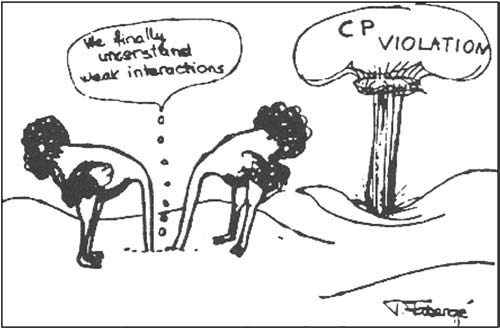
\includegraphics[scale=0.7]{Immagini/vignetta}
\caption{Vignetta presentata da Nicola Cabibbo nel 1966. La violazione di CP, non prevista dai modelli di \emph{quark mixing} teorizzati fino ad allora, viene rappresentata come una potente esplosione, in grado di scuotere le fondamenta della fisica teorica dell'epoca.}
\end{center}
\end{figure}

\subsection{Teoria di Cabibbo}
\noindent
Nel 1963, N. Cabibbo ipotizzò che una rottura spontanea della simmetria portasse ad un $mixing$ dei campi $d_L$ ed $s_L$, portando ad una
espressione della corrente carica della forma:
\begin{equation}\label{Cab}
 J^1_{\mu} + iJ^2_{\mu} = \bar{u}_L\gamma_\mu (\cos(\theta)d_L + \sin(\theta)s_L)
\end{equation}
dove $\theta$ viene detto angolo di Cabibbo. Questa ipotesi, unita ad alcune considerazioni derivanti dalla teoria delle interazioni forti, 
permise di ottenere un ottimo accordo con i dati sperimentali riguardanti le disintegrazioni $\beta$ di adroni con e senza stranezza.
Tuttavia questa teoria permette l'esistenza di correnti deboli neutre con cambiamento di sapore (cioè di stranezza, in questo semplice schema
a tre quark), il che è in contrasto con i dati sperimentali \cite{Maiani}. Infatti la \eqref{Cab} può essere riscritta nel modo seguente:
\begin{equation}
  J^1_{\mu} + iJ^2_{\mu} = \bar{q}_L C \gamma_\mu q_L = \bar{q}_L \Bigg(\begin{matrix} 0 & \cos(\theta) & \sin(\theta) \\ 0 & 0 & 0 \\ 0 & 0 & 0 \end{matrix}\Bigg) \gamma_\mu q_L
\end{equation}
È possibile dimostrare che la corrente elettrodebole neutra coinvolge il commutatore $[C, C^{\dag}]$. Se questo risulta essere non diagonale, 
sono possibili correnti deboli con cambiamento di sapore. Nel caso sopra esposto si ha:
\begin{equation}
 [C, C^{\dag}] = \Bigg(\begin{matrix} 1 & 0 & 0 \\ 0 & -\cos^2(\theta) & -sin(\theta)\cos(\theta) \\ 0 & -\sin(\theta)\cos(\theta) & -\sin^2(\theta) \end{matrix}\Bigg)
\end{equation}

\subsection{Teoria di Glashow, Iliopoulos e Maiani}
\noindent
La difficoltà insita nella teoria di Cabibbo venne superata nel 1970 con l'ipotesi dell'esistenza di un quarto quark, oggi chiamato $charm$,
avente le stesse proprietà elettrodeboli del quark $up$.
In questo modo, i campi \emph{left-handed} dei quark $up$ e $down$ continuano a formare un doppietto elettrodebole, un secondo doppietto è formato
dai campi \emph{left-handed} dei quark $charm$ e $strange$, mentre gli altri campi rappresentano singoletti elettrodeboli:
\begin{equation}
 \binom{u}{d}_L;\;\binom{c_L}{s_L}_L;\;u_R;\;d_R;\;c_R;\;s_R
\end{equation}
Ora $C$ è una matrice $4×4$ e la corrente debole carica prende la forma:
\begin{equation}
 J^1_{\mu} + iJ^2_{\mu} = \bar{q}_L \Bigg(\begin{matrix} 0 & U_{GIM} \\ 0 & 0 \end{matrix}\Bigg)
\end{equation}
dove si è indicata con $U_{GIM}$ la matrice:
\begin{equation}
U_{GIM} = \Bigg(\begin{matrix} \cos(\theta) & \sin(\theta) \\ -\sin(\theta) & \cos(\theta) \end{matrix}\Bigg)
\end{equation}
A causa dell'unitarietà di $U_{GIM}$, il commutatore $[C. C^{\dag}]$ è completamente diagonale:
\begin{equation}
 [C. C^{\dag}] = \Bigg(\begin{matrix} U_{GIM}U_{GIM}^\dag & 0 \\ 0 & -U_{GIM}^\dag U_{GIM} \end{matrix}\Bigg) = \Bigg(\begin{matrix} 1 & 0 \\ 0 & -1 \end{matrix}\Bigg)
\end{equation}
quindi, in accordo con i dati sperimentali, non sono consentite correnti elettrodeboli neutre con cambiamento di sapore \cite{Maiani}.

\subsection{Teoria di Kobayashi-Maskawa}
\noindent
Nel 1973 la validità del meccanismo di Glashow, Iliopoulos e Maiani e la conseguente esistenza del quark $charm$ erano ampiamente accettate dai fisici
teorici. Tuttavia la violazione di CP, osservata per la prima volta nel decadimento dei kaoni neutri nel 1964 e che da allora
era stata ampiamente studiata, non era prevista da tale meccanismo.
Il modo più naturale per avere una violazione di CP è quello di avere una fase complessa all'interno della matrice di \emph{mixing}\cite{Kobayashi}.
Tuttavia è immediato verificare che una eventuale fase complessa presente nella matrice $U_{GIM}$ può sempre essere eliminata sfruttando 
l'arbitrarietà nella fase del campo associato a ciascun quark.
Kobayashi e Maskawa calcolarono la dimensione minima che una matrice di \emph{mixing} doveva possedere affinché risultasse impossibile eliminare
tutte le fasi.
\begin{teorema}
Una matrice di \emph{mixing} $V$ di dimensione $N$ contiene $\frac{1}{2}(N-1)(N-2)$ fasi irriducibili.
\end{teorema}
\begin{proof}
 Una generica matrice complessa $N × N$ contiene $2N^2$ parametri. La condizione di unitarietà implica:
\begin{equation}
 \sum_j V_{ij}V_{jk}^* = \delta_{ik}
\end{equation}
Attraverso queste relazioni è possibile eliminare $N^2$ parametri, ottenendo un totale di $N^2$ parametri indipendenti restanti.
Le fasi dei campi associati ai quark possono essere ruotate liberamente. La trasformazione:
\begin{equation}
 V \rightarrow \begin{bmatrix} e^{-i\phi_1^u} & \cdots & 0 \\ \vdots & \ddots & \vdots \\ e^{-i\phi_N^u} & \cdots & 0\end{bmatrix} V \begin{bmatrix} e^{i\phi_1^d} & \cdots & 0 \\ \vdots & \ddots & \vdots \\ e^{i\phi_N^d} & \cdots & 0\end{bmatrix}
\end{equation}
in cui $V$ viene moltiplicata a destra ed a sinistra da una matrice diagonale contenente fattori di fase, non ha effetti fisici.
Dato che la fase complessiva è arbitraria, è possibile eliminare $2N-1$ fasi relative. In questo modo, $V$ risulta contenere $(N-1)^2$ 
parametri fisici indipendenti.
Inoltre, una generica matrice ortogonale di dimensione $N$ contiene $\frac{1}{2}N(N-1)$ angoli di rotazione. Per cui, in definitiva, 
il numero di fasi irriducibili in una matrice di \emph{mixing} $N × N$ è dato da:
\begin{equation}
 n_{fasi} = (N-1)^2 - \frac{1}{2}N(N-1) = \frac{1}{2}(N-1)(N-2)
\end{equation}
\end{proof}
Dal teorema precedente deriva che con due famiglie di quark (come previsto dalla teoria di Glashow, Iliopoulos e Maiani) non si hanno fasi irriducibili:
\begin{equation}
 n_{fasi} = \frac{1}{2} (2-1)(2-2) = 0 
\end{equation}
Per questo motivo Kobayashi e Maskawa ipotizzarono l'esistenza di una terza famiglia di quark, in maniera tale che la matrice di mixing contenga:
\begin{equation}
 n_{am} = \frac{1}{2}N(N-1) = 3
\end{equation}
angoli di \emph{mixing}, che con tre famiglie di quark possono essere rappresentati con gli angoli di Eulero e 
\begin{equation}
 n_{fasi} = \frac{1}{2}(N-1)(N-2) = 1
\end{equation}
fase irriducibile, che inserisce nel quadro teorico delle interazioni elettrodeboli la violazione di CP \cite{Maiani}.
La matrice di \emph{mixing} per tre famiglie di quark viene chiamata \emph{matrice CKM}, dalle iniziali di Cabibbo (che per primo introdusse
l'idea del \emph{quark mixing}) Kobayashi e Maskawa:
\begin{equation}
  V_{CKM} = \begin{bmatrix} V_{ud} & V_{us} & V_{ub} \\ V_{cd} & V_{cs} & V_{cb} \\ V_{td} & V_{ts} & V_{tb}\end{bmatrix}
\end{equation}
Esistono varie rappresentazioni di questa matrice. La più usata al giorno d'oggi è dovuta a Wolfenstein ed è data dalla seguente espressione:
\begin{equation}
  V_{CKM} = \begin{bmatrix} 1-\frac{\lambda^2}{2} - \frac{\lambda^4}{8}& \lambda & A\lambda^3(\rho - i\eta) \\ -\lambda + \frac{A^2(1-2\rho)}{2}\lambda^5 - iA^2\eta\lambda^5 & 1-\frac{\lambda^2}{2} - (\frac{1}{8}+ \frac{A^2}{2})\lambda^4& A\lambda^2 \\ A\lambda^3[1-(1-\frac{\lambda^2}{2})(\rho + i\eta)]] & -A\lambda^2(1-\frac{\lambda^2}{2})[1+\lambda^2(\rho + i\eta)] & 1- \frac{A^2\lambda^4}{2}\end{bmatrix} + O(\lambda^6)
\end{equation}
Dove $\lambda$ è il seno dell'angolo di Cabibbo. Attualmente le migliori stime dei parametri $\lambda$, $A$, $\rho$ ed $\eta$ sono:
\begin{equation}
\lambda = 0,2257^{+0,0009}_{-0,0010} 
\end{equation}
\begin{equation}
A = 0,814^{+0,021}_{-0,022} 
\end{equation}
\begin{equation}
\rho = 0,135^{+0,031}_{-0,016} 
\end{equation}
\begin{equation}
\eta = 0,349^{+0,015}_{-0,017} 
\end{equation}
Questa rappresentazione ha il grande vantaggio di mettere in luce la struttura gerarchica della matrice CKM. Le ampiezze di transizione risultano infatti di ordine 
zero sulla diagonale (viene cioè favorita la transizione di ciascun quark di tipo $down$ nel quark di tipo $up$ della stessa famiglia e viceversa), mentre le altre 
transizioni vengono, in diversa misura, sfavorite.


\section{Determinazione dei parametri della matrice CKM}
\noindent
La martice CKM è data dall'espressione:
\begin{equation}
 V_{CKM} = \begin{bmatrix} V_{ud} & V_{us} & V_{ub} \\ V_{cd} & V_{cs} & V_{cb} \\ V_{td} & V_{ts} & V_{tb}\end{bmatrix}
\end{equation}
I moduli dei parametri della matrice CKM possono essere ricavati in maniera empirica. Di seguito vengono elencati i valori di tutti gli elementi e i processi fisici sfruttati
per la loro misurazione \cite{Sozzi}:
\begin{enumerate}
\item $|V_{ud}| = 0,97428 \pm 0,00015$ può essere ricavato come la radice quadrata del rapporto tra i ratei dei decadimenti nucleari $\beta$ del tipo di Fermi ($J^{p} = 0^+ \rightarrow 0^+$)
 e il decadimento del muone:
\begin{equation}
 |V_{ud}|^2 = \frac{\sigma(d \rightarrow u e^- \bar{\nu_e})}{\sigma(\mu^-\rightarrow e^- \bar{\nu_e} \nu_{\mu})}
\end{equation}
\item $|V_{us}| = 0,2253 \pm 0,0007$ (angolo di Cabibbo) può essere ricavato come la radice quadrata del rapporto tra il rateo del decadimento semileptonico del kaone positivo $K^+$ e del muone:   
\begin{equation}
|V_{us}|^2 = \frac{\sigma(K^+ \rightarrow \pi^{0} e^{+} \nu_{e})}{\sigma(\mu^-\rightarrow e^- \bar{\nu_e} \nu_{\mu})}
\end{equation}
\item $|V_{cb}| = 0,0410^{+0,0011}_{-0,0007}$ può essere ricavato come la radice quadrata del rapporto tra i ratei dei decadimenti del ${B_d}^0$ e del muone:   
      \begin{equation}
       |V_{cb}|^2 = \frac{\sigma({B^0}_d \rightarrow D^{*-} l^+ \nu_l)}{\sigma(\mu^-\rightarrow e^- \bar{\nu_e} \nu_{\mu})}
      \end{equation}
      dove $l$ può indicare uno qualunque dei simboli $e$, $\mu$ o $\tau$.

\item $|V_{ub}| = 0,00347^{0,00016}_{0,00012}$ può essere ricavato dallo studio dei decadimenti del mesone ${B_d}^0$, conoscendo il valore di $|V_{cb}|$:
      \begin{equation}
      \bigg(\frac{|V_{ub}|}{|V_{cb}|}\bigg)^2 = \frac{\sigma({B^0}_d \rightarrow D^{*-} l^+ \nu_l)}{\sigma({B^0}_d \rightarrow \pi^{-} l^+ \nu_l)}
      \end{equation}
\item $|V_{cd}| = 0,2252 \pm 0,0007$ viene determinato dalla reazione di produzione di $charm$ attraverso scattering fortemente anelastici di neutrini muonici sui nuclei, 
      secondo la reazione:
       \begin{equation}
       \nu_{\mu} d \rightarrow c \mu^-
       \end{equation}
       seguita dalla reazione:
      \begin{equation}
       c \rightarrow d \mu^+ \bar{\nu_{\mu}}
      \end{equation}
      (l'osservazione di antimuoni in seguito all'interazione di un fascio di neutrini muonici con la materia nucleare indica che è avvenuta produzione di $charm$)
\item $|V_{cs}| = 0,97345^{+0,00015}_{-0,00016}$ può essere ricavato anch'esso dalla reazione di produzione di charm attraverso lo scattering 
       di neutrini, oppure dalle reazioni di decadimento del mesone $D$ in particelle strane e dal decadimento $charm$ dei bosoni $W$.
\item $|V_{td}| = 0,00862^{+0,00026}_{-0,00020}$ viene ricavato dalle oscillazioni $B^0_d \longleftrightarrow \bar{B^0_d}$, nelle quali il $top$ entra come particella virtuale,
      è possibile infatti dimostrare:
      \begin{equation}
       \delta m_{B^0_d} \alpha \frac{{m_t}^2}{{m_W}^2} m_{B^0_d}|V_{td}|^2
      \end{equation}
\item $|V_{ts}| = 0,0403^{+0,0011}_{-0,0007}$ può essere ricavato sfruttando le oscillazioni $B^0_d \longleftrightarrow \bar{B^0_d}$ e $B^0_s \longleftrightarrow \bar{B^0_s}$, vale infatti la relazione:
	\begin{equation}
	 \frac{\Delta m_{B^0_d}}{\Delta m_{B^0_s}} \approx \frac{|V_{td}|^2}{|V_{ts}|^2}
	\end{equation}
\item $|V_{tb}| = 0,999152^{+0,000030}_{-0,000045}$ può essere stimato in maniera approssimativa dalla reazione di decadimento del $top$:
      \begin{equation}
       t \rightarrow b l \bar{\nu}_l
      \end{equation}
      dove si è adottata nuovamente la notazione $l = e$, $\mu$ o $\tau$.
\end{enumerate}
\begin{figure}
\begin{center}
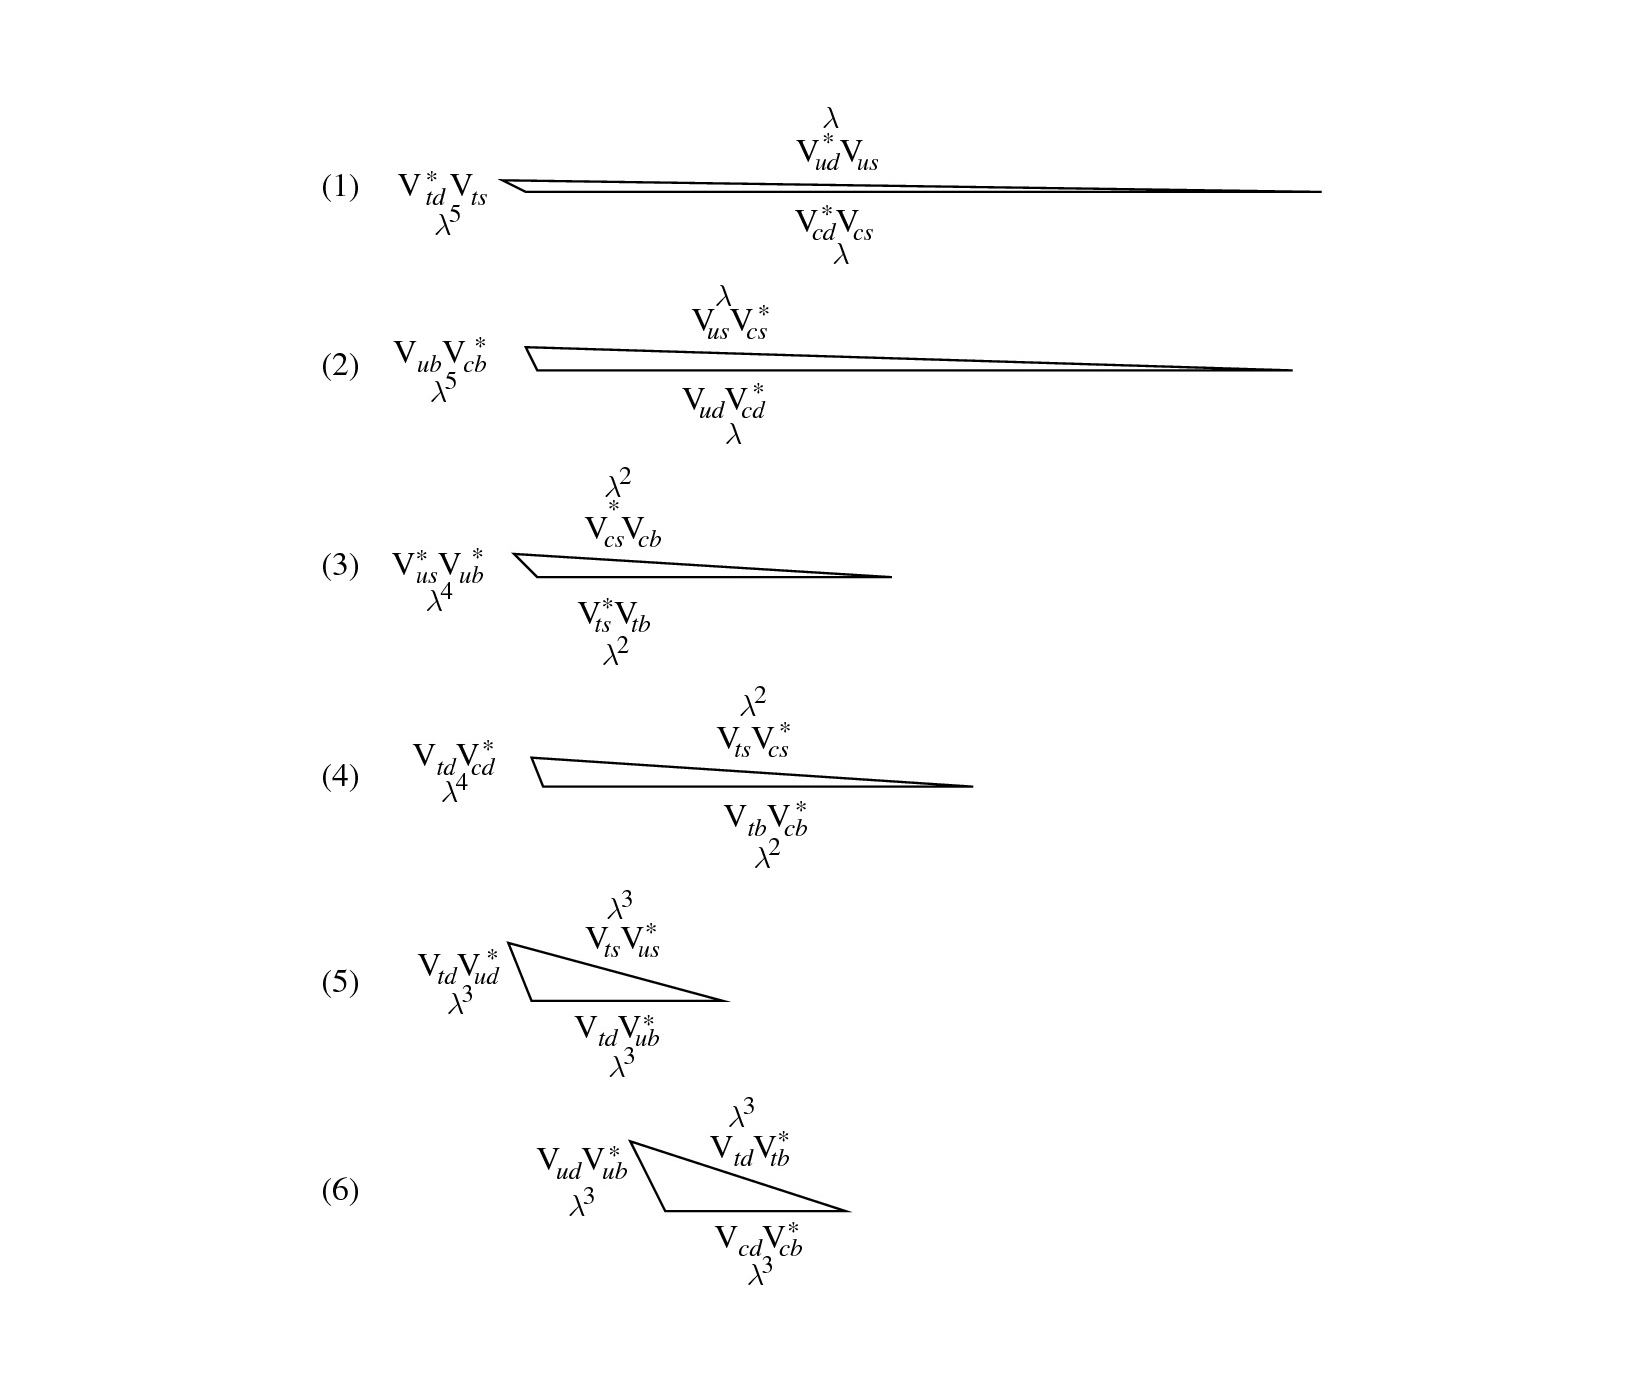
\includegraphics[scale=0.18]{Immagini/triangoli}
\caption{I sei triangoli di unitarietà}
\end{center}
\end{figure}
\section{Triangoli di unitarietà}
\noindent
L'unitarietà della matrice CKM equivale alla validità delle dodici espressioni:
\begin{equation}
  \sum_j V_{ij}V_{jk}^* = \delta_{ik}
\end{equation}
Queste condizioni possono anche essere viste come:
\begin{enumerate}
 \item $6$ relazioni di normalizzazione sulle ampiezze di transizione, cioè la richiesta che la somma dei moduli quadri di tutti gli elementi appartenenti alla stessa riga (colonna) sia pari ad uno:
    \begin{equation}
     \sum_j V_{ij}V_{ji}^* = |V_{ij}|^2 = 1
    \end{equation}
 \item $6$ relazioni di ortogonalità, cioè la richiesta che ogni vettore riga (colonna) sia ortogonale agli altri vettori riga (colonna):
    \begin{equation}
     \sum_j V_{ij}V_{jk}^* = 0 \ \ \ \ \ \ \ \ \ \ \ (i\neq j)
    \end{equation}

\end{enumerate}
Le relazioni di ortogonalità ammettono una immediata interpretazione geometrica: rappresentano infatti sei triangoli nel piano complesso, i cosiddetti \emph{triangoli di unitarietà}.
I lati e gli angoli di questi triangoli non dipendono dalla fase dei campi associati ai quark e sono quindi fisicamente misurabili. Essi rappresentano un ottimo terreno
per testare la validità del Modello Standard, almeno per quanto riguarda le interazioni elettrodeboli. Infatti, se dalla misura dei parametri caratteristici di questi triangoli
sorgessero delle inconsistenze (cioè, ad esempio, se un lato fosse maggiore della somma degli altri due, o se la somma degli angoli interni non fosse pari all'angolo piatto, 
o ancora se i valori degli angoli fossero incompatibili con quelli misurati per i lati, etc...) se ne dedurrebbe che la matrice CKM non è unitaria, con conseguente
crollo del Modello Standard e la scoperta di Nuova Fisica \cite{BigiSanda}.
In seguito si elencheranno i sei triangoli di unitarietà, indicando l'ordine in $\lambda$ di ciascun lato:
\begin{enumerate}
 \item \begin{equation}
\begin{matrix} \underbrace{V_{ud}^*V_{us}}_{O(\lambda)} \end{matrix} \begin{matrix} {+}\\{ } \end{matrix} \begin{matrix} \underbrace{V_{cd}^*V_{cs}}_{O(\lambda)} \end{matrix} \begin{matrix} {+}\\{ } \end{matrix} \begin{matrix} \underbrace{V_{td}^*V_{ts}}_{O(\lambda^5)} \end{matrix} \begin{matrix} {=}\\{ } \end{matrix} \begin{matrix} {0}\\{ } \end{matrix}
 \end{equation}
 \item \begin{equation}
\begin{matrix} \underbrace{V_{ud}V_{cd}^*}_{O(\lambda)} \end{matrix} \begin{matrix} {+}\\{ } \end{matrix} \begin{matrix} \underbrace{V_{us}V_{cs}^*}_{O(\lambda)} \end{matrix} \begin{matrix} {+}\\{ } \end{matrix} \begin{matrix} \underbrace{V_{ub}V_{cb}^*}_{O(\lambda^5)} \end{matrix} \begin{matrix} {=}\\{ } \end{matrix} \begin{matrix} {0}\\{ } \end{matrix}
 \end{equation}
 \item \begin{equation}
\begin{matrix} \underbrace{V_{us}^*V_{ub}}_{O(\lambda^4)} \end{matrix} \begin{matrix} {+}\\{ } \end{matrix} \begin{matrix} \underbrace{V_{cs}^*V_{cb}}_{O(\lambda^2)} \end{matrix} \begin{matrix} {+}\\{ } \end{matrix} \begin{matrix} \underbrace{V_{ts}^*V_{tb}}_{O(\lambda^2)} \end{matrix} \begin{matrix} {=}\\{ } \end{matrix} \begin{matrix} {0}\\{ } \end{matrix}
 \end{equation}
 \item \begin{equation}
\begin{matrix} \underbrace{V_{td}V_{cd}^*}_{O(\lambda^4)} \end{matrix} \begin{matrix} {+}\\{ } \end{matrix} \begin{matrix} \underbrace{V_{ts}V_{cs}^*}_{O(\lambda^2)} \end{matrix} \begin{matrix} {+}\\{ } \end{matrix} \begin{matrix} \underbrace{V_{tb}V_{cb}^*}_{O(\lambda^2)} \end{matrix} \begin{matrix} {=}\\{ } \end{matrix} \begin{matrix} {0}\\{ } \end{matrix}
 \end{equation}
 \item \begin{equation}
\begin{matrix} \underbrace{V_{td}V_{ud}^*}_{O(\lambda^3)} \end{matrix} \begin{matrix} {+}\\{ } \end{matrix} \begin{matrix} \underbrace{V_{ts}V_{us}^*}_{O(\lambda^3)} \end{matrix} \begin{matrix} {+}\\{ } \end{matrix} \begin{matrix} \underbrace{V_{tb}V_{ub}^*}_{O(\lambda^3)} \end{matrix} \begin{matrix} {=}\\{ } \end{matrix} \begin{matrix} {0}\\{ } \end{matrix}
 \end{equation}
 \item \begin{equation}
\begin{matrix} \underbrace{V_{ud}V_{ub}^*}_{O(\lambda^3)} \end{matrix} \begin{matrix} {+}\\{ } \end{matrix} \begin{matrix} \underbrace{V_{cd}V_{cb}^*}_{O(\lambda^3)} \end{matrix} \begin{matrix} {+}\\{ } \end{matrix} \begin{matrix} \underbrace{V_{td}V_{tb}^*}_{O(\lambda^3)} \end{matrix} \begin{matrix} {=}\\{ } \end{matrix} \begin{matrix} {0}\\{ } \end{matrix}
 \end{equation}
\end{enumerate}
Osservando la geometria di questi triangoli, è possibile riunirli in tre diverse categorie:
\begin{enumerate}
 \item I primi due triangoli sono estremamente ``schiacciati``: due lati sono di ordine $\lambda$, metre il terzo di ordine $\lambda^5$, cioè circa $\lambda^4 \approx 2,3 \cdot 10^{-3}$
volte più piccolo. 
 \item Il terzo ed il quarto triangolo sono hanno anch'essi lati di lunghezza molto diseguale, ma non in maniera così marcata.
 \item Gli ultimi due hanno i lati dello stesso ordine di grandezza, ragion per cui i loro angoli sono tutti particolarmente ampi, nell'ordine del radiante.
\end{enumerate}

Nello studio della martice CKM, un particolare interesse ricopre il triangolo dato dall'espressione:
\begin{equation}
 V_{ud}V_{ub}^* + V_{cd}V_{cb}* + V_{td}V_{tb}^* = 0
\end{equation}
A cui spesso ci si riferisce nella letteratura sull'argomento come \emph{il triangolo di unitarietà}, per antonomasia \cite{Branco}.
I parametri attraverso i quali viene definito questo triangolo di unitarietà sono quantità importanti nella dinamica del decadimento del $B$ e nelle oscillazioni $B_d - \bar{B_d}$.
È possibile dimostrare dunque attraverso la matrice CKM che le transizioni deboli che coinvolgono il quark $beauty$ sono dell'ordine dell'unità.
Utilizzando la parametrizzazione di Wolfenstein i lati di questo triangolo risultano essere:
\begin{equation}
V_{ud}V_{ub}^* = -A\lambda^3
\end{equation}
\begin{equation}
V_{cd}V_{cb}* = A\lambda^3 (\bar{\rho} + i\bar{\eta})
\end{equation}
\begin{equation}
 V_{td}V_{tb}^* = A\lambda^3 (1-\bar{\rho}-i\bar{\eta})
\end{equation}
Mentre gli angoli sono:
\begin{equation}
 \alpha = \arg \Big(-\frac{V_{td}V^*_{td}}{V_{ud}V^*_{ub}}\Big)
\end{equation}
\begin{equation}
 \beta = \arg \Big(-\frac{V_{cd}V^*_{cb}}{V_{td}V^*_{tb}}\Big)
\end{equation}
\begin{equation}
 \gamma = \arg\Big(-\frac{V_{ud}V_{ub}^*}{V_{cd}V_{cb}^*}\Big)
\end{equation}
Dato che il seno dell'angolo di Cabibbo $\lambda$ ed il parametro $A$ sono noti con grande precisione, risulta conveniente eseguire una trasformazione di scala
che elimini i fattori $A\lambda^3$, in modo da potersi limitare alla misura di $\rho$ ed $\eta$ \cite{BigiSanda}. Con questa riparametrizzazione uno dei vertici risulta avere coordinate 
$(\bar{\rho},\bar{\eta})$. La misura sperimentale dei parametri esatti di questo triangolo è uno dei problemi aperti più attuali della fisica delle alte energie.
In particolare, nelle parti successive ci si concentrerà sulla misura dell'angolo $\gamma$.
\begin{figure}
\begin{center}
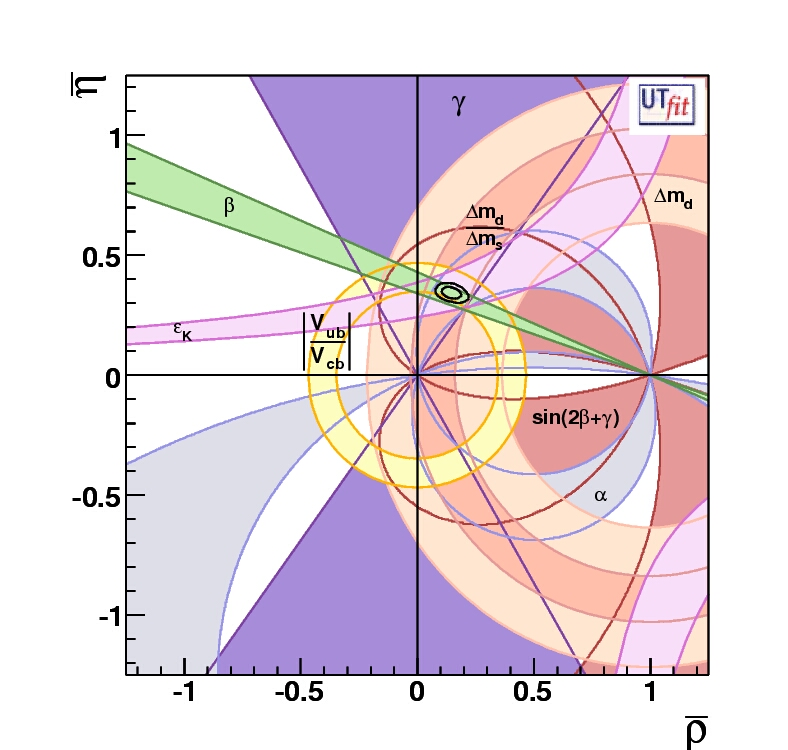
\includegraphics[scale=0.4]{Immagini/triangoloUTfit}
\caption{Lo stato attuale delle misure dei parametri del triangolo di unitarietà. Tutte le misure sono in ottimo accordo con le previsioni teoriche. (\emph{UTfit collaboration, 2012})}
\end{center}
\end{figure}